\begin{figure}[t!]
  \centering
  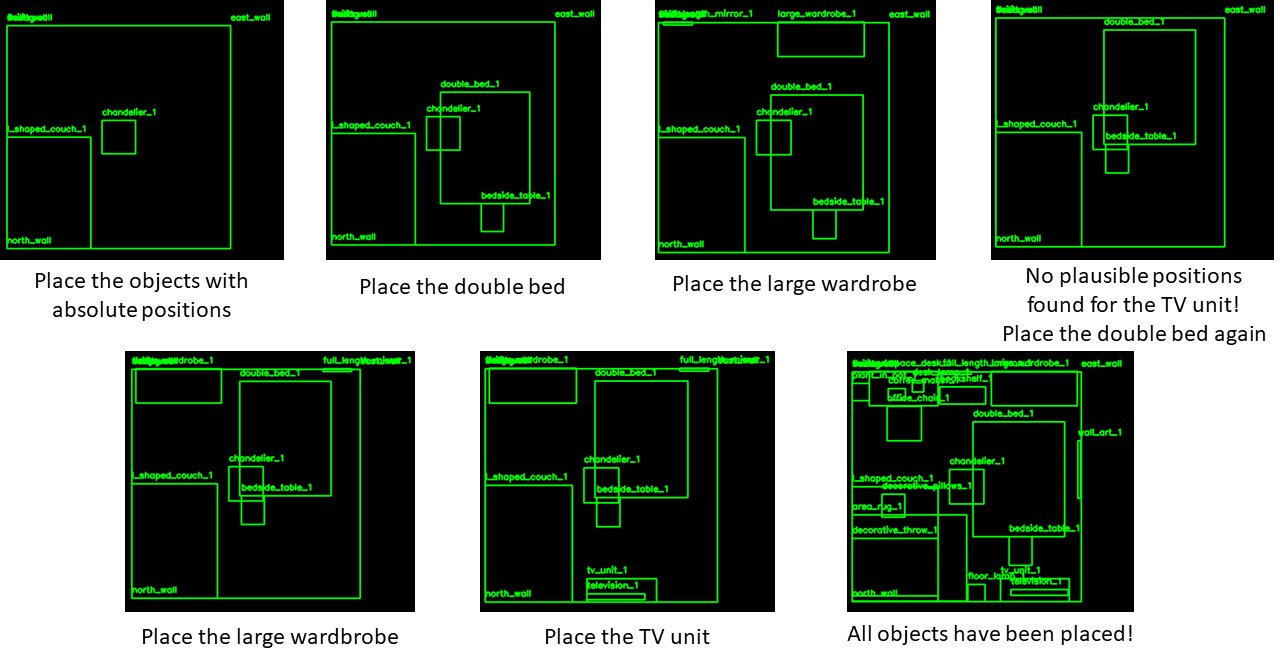
\includegraphics[width=1.0\textwidth]{images/backtracking.png}
  \caption{
    \textbf{Backtracking-based Scene Graph Layout.}
    Starting from the scene graph specifying interior items as nodes connected with relative relationships, the backtracking algorithm solves for their absolute placement in the room. The algorithm reverses dead-end configurations and excels at object placement while respecting spatial constraints.
  }
  \label{fig:backtracking}
\end{figure}
